\documentclass[journal]{IEEEtran}

\usepackage{amsmath,amssymb}
\usepackage{graphicx}
\usepackage{booktabs}
\usepackage{multirow}
\usepackage{cite}
\usepackage{url}
\usepackage{xcolor}
\usepackage{array}
\usepackage{subcaption}
\usepackage{hyperref}

\graphicspath{{figures/}}

\title{Content-Adaptive Diffusion Steganography with\\
Spectral and Adversarial Regularisation}

\author{Anonymous Authors% <-this % stops a space
\thanks{Manuscript prepared for submission. Source code, training
artifacts, and evaluation scripts are available in the project
repository.}}

\markboth{IEEE Transactions}{Anonymous \MakeLowercase{\textit{et al.}}: Content-Adaptive Diffusion Steganography}

\begin{document}

\maketitle

\begin{abstract}
We present DSCSP, a diffusion-based image-steganography framework that
hides a fixed-length payload inside covers produced by a frozen
denoising diffusion sampler. The system is composed of three trainable
modules---a content-adaptive perturbation controller, a spatial
extractor with a ResNet backbone, and a spectrally-regularised
discriminator augmented with Spatial Rich Model (SRM) filters. We
describe four generations of the controller design, starting from a
tiled parameter lookup and converging on a three-level U-Net that
fuses image content with two parallel payload-carrier branches. The
controller is trained together with the extractor through a short
bootstrap stage followed by an adversarial phase that uses a
JPEG-heavy differentiable attack layer, an FFT-magnitude spectral
loss, and an LPIPS perceptual term. We then expose the trade-off
surface of the resulting system through an eleven-cycle refinement
schedule that sweeps four training recipes. Our primary operating point (cycle~9) achieves a clean bit-error rate
of $1.95\!\times\!10^{-5}$ and a JPEG~Q75 bit-error rate of
$3.91\!\times\!10^{-5}$ at $30.68\,\mathrm{dB}$ PSNR, establishing
the headline recovery result; a detectability-focused variant further
reduces adaptive-steganalysis AUC to $0.6915$, illustrating the
accessible trade-off surface available from a single shared
architecture. Supporting
analyses on a later exploratory variant measure residual statistical
structure through Inception-feature divergence, radial power-spectrum
tests, and singular-value concentration. We also report
cross-dataset behaviour on CIFAR-10 and STL-10 and discuss the
trade-off between decoding fidelity, imperceptibility, and
resilience to geometric distortion that shapes the remaining design
space.
\end{abstract}

\begin{IEEEkeywords}
Image steganography, diffusion models, steganalysis, adversarial
training, spectral analysis, robustness.
\end{IEEEkeywords}

\section{Introduction}
\IEEEPARstart{G}{enerative} diffusion models~\cite{ho2020denoising,
song2020denoising} now produce image distributions whose statistics
we can engineer by design. We use that property to sidestep a core
limitation of cover-modification steganography: rather than modifying
a natural photograph whose statistics the sender cannot control, we
generate the cover from a frozen sampler that sender and receiver
share. The payload enters the channel as a bounded perturbation of
that generated cover.

Realising this in practice means resolving three tensions that rarely
align. The receiver must decode the payload after the image has
passed through compression, resampling, and additive noise. We must
keep the stego image within the same statistical distribution an
honest sampler would produce, because an adaptive detector trained on
both classes will otherwise separate them. The embedding must also
remain perceptually transparent. Designing the system is largely the
act of deciding which of these three objectives to compromise, and
by how much.

This paper documents the current state of DSCSP (Diffusion-Stego with
Conditional Sampling Paths), a research codebase that has progressed
through four architectural generations and a short exploratory fifth
branch. The common structure is a frozen denoising diffusion sampler
that produces covers, followed by a trainable controller that adds a
small perturbation conditioned on both the cover and the payload. An
extractor reads the payload back from the stego image, and a
spectrally-normalised discriminator keeps the perturbation
statistically inconspicuous. The controller has evolved from a tiled
parameter lookup~(v1/v2) through a quality-tuned refinement~(v3) into
the content-adaptive U-Net used in the current system~(v4). The v5
branch adds a redundant-coding stage and an SRM feature-matching loss;
we use it only to provide supporting statistical evidence, not as the
primary result.

We make the following contributions:

\begin{itemize}
    \item We describe the current DSCSP pipeline in detail,
    including the two explicit payload-carrier paths that were
    introduced to give the system a stable bit-transport route, the
    spatial extractor head that replaced the older bottleneck, and
    the SRM-assisted discriminator used during adversarial training.
    \item We present a training recipe that combines a short
    extractor and controller bootstrap with an adversarial phase
    built around a differentiable JPEG proxy, a radial-spectral
    regulariser, and an LPIPS perceptual term.
    \item We report an eleven-cycle refinement sweep that exposes a
    clear frontier between decoding recovery and adaptive
    detectability, and show that different operating points along
    this frontier are accessible without changing the underlying
    architecture.
    \item We complement the quantitative metrics with an independent
    statistical-analysis pass that combines Inception-feature
    divergence, radial power-spectrum comparison, and
    singular-value concentration of the mean perturbation, and we
    use those probes to characterise the residual signatures of the
    current system.
    \item We analyse cross-dataset behaviour on CIFAR-10 and STL-10
    and identify crop-resize as the distortion class for which the
    current extractor design does not yet amortise a spatial
    signal. We treat that observation as a direction for future
    work rather than an isolated failure, and we discuss design
    choices that could reshape the trade-off surface.
\end{itemize}

The rest of the paper is organised as follows. Section~\ref{sec:rw}
reviews related work on learned steganography, diffusion-based
hiding, and modern steganalysis. Section~\ref{sec:setup} specifies
the threat model. Section~\ref{sec:arch} describes the system after
its four generations of changes. Section~\ref{sec:training} describes
the training strategy and evaluation protocol.
Section~\ref{sec:experiments} reports the quantitative results and
Section~\ref{sec:ablations} the ablation evidence.
Section~\ref{sec:security} presents the statistical analysis.
Section~\ref{sec:discussion} discusses trade-offs and open directions
before concluding in Section~\ref{sec:conclusion}.

\section{Related Work}
\label{sec:rw}

\subsection{Classical and Learned Image Steganography}
Classical schemes such as HUGO, WOW, and the UNIWARD
family~\cite{pevny2010using, holub2012designing, holub2014universal}
define a hand-crafted distortion function that favours textured and
noisy regions. They remain a strong baseline for low-payload
regimes, but they were designed for a setting in which the cover is
a photograph with fixed statistics, and they do not naturally
incorporate a learned decoder.

Encoder--decoder networks removed that restriction.
HiDDeN~\cite{zhu2018hidden} jointly optimises an encoder, a decoder,
and a differentiable channel model and shows that message recovery
under mild distortions can be learned end-to-end.
SteganoGAN~\cite{zhang2019steganogan} pushes capacity through an
adversarial term that discourages detectable artefacts, and several
later systems refined the idea using perceptual losses, attention, and
attack ensembles. These works established the value of optimising
embedding and recovery jointly and of exposing the pipeline to an
attack channel during training. DSCSP inherits both conventions.

\subsection{Diffusion-Based Steganography and Generative Covers}
A more recent line of work pushes steganography into the generative
process itself. Diffusion-Stego~\cite{wei2023diffusionstego} maps the
payload into the initial noise of a diffusion sampler and recovers it
through an inverted trajectory. LDStega~\cite{zhang2024ldstega} works
inside a latent diffusion model, and DERO~\cite{zhao2024dero} shows
that diffusion-based watermarks can remain legible through generative
erasure attacks. These schemes are training-free or nearly
training-free, and they bind the message tightly to the sampling
trajectory. DSCSP is a complementary design: the diffusion backbone
is used as a frozen source of cover distributions, and the learned
perturbation is applied in image space. This separation makes it
easier to change the attack channel and the discriminator without
retraining the sampler, but it inherits the full attack surface of
image-space embedding.

\subsection{Modern Steganalysis}
The relevant attacker family is a learned steganalyser trained on the
same image distribution as the sender. Classical
SRM~\cite{fridrich2012rich} extracts noise residuals through fixed
high-pass filters and remains a strong feature basis.
SRNet~\cite{boroumand2019deep} demonstrated that deep networks
trained end-to-end on raw pixels can match or exceed SRM in realistic
regimes. DSCSP's discriminator combines both views: it prepends SRM
filters to a spectrally-normalised CNN so that the adversarial
gradient amplifies high-frequency residuals during training. In
addition, we report results against an independent adaptive
steganalyser whose training mirrors the channel model used at test
time.

\subsection{Forensics of Diffusion Imagery}
Detection of diffusion-generated imagery is a live research
area~\cite{corvi2023detection}. Because DSCSP produces covers by
sampling from a frozen diffusion model, an attacker who can reliably
distinguish diffusion images from natural photographs retains an
additional channel beyond steganalysis proper. We consider that a
separate threat and do not evaluate against a dedicated diffusion
detector in this paper.

\section{Threat Model and Problem Setup}
\label{sec:setup}

\subsection{Actors}
Sender and receiver share the frozen diffusion sampler, the
controller $C_\phi$, the extractor $E_\psi$, and a seed or noise
latent. Given a payload $b\in\{0,1\}^{L}$ with $L=256$, the sender
produces a cover $x_c\in\mathbb{R}^{3\times 256\times 256}$ via
DDIM~\cite{song2020denoising} sampling and emits
\begin{equation}
x_s \;=\; \mathrm{clip}\!\left(x_c + C_\phi(x_c, b),\; -1,\; +1\right).
\label{eq:embed}
\end{equation}
The receiver observes $\mathcal{A}(x_s)$ after a channel
$\mathcal{A}$ and decodes $\hat{b}=\mathrm{sign}(E_\psi(\mathcal{A}(x_s)))$.
Figure~\ref{fig:system} summarises this pipeline.

\begin{figure*}[t]
\centering
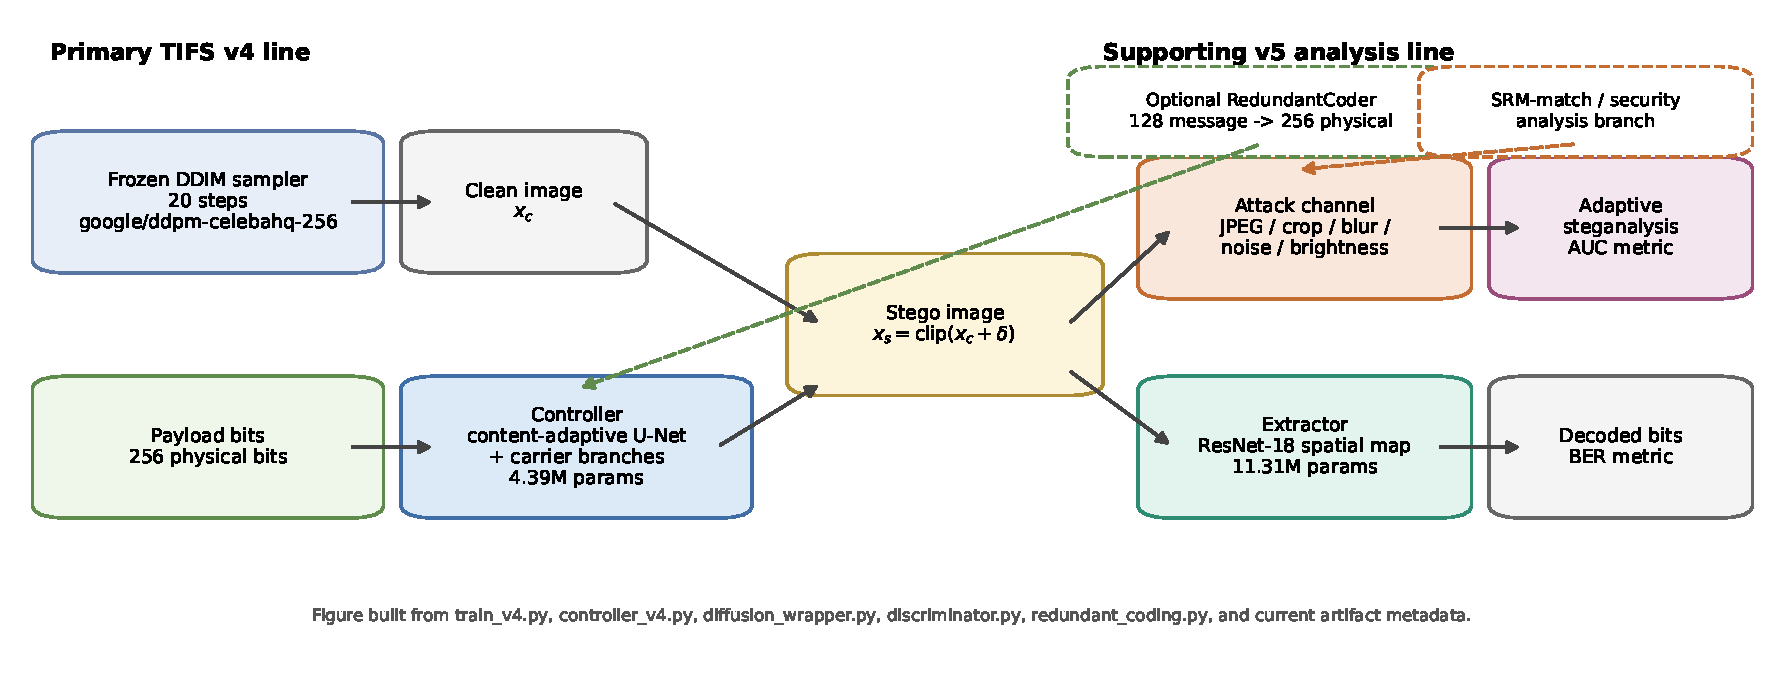
\includegraphics[width=0.95\textwidth]{system_overview.pdf}
\caption{System overview. A frozen DDPM is used as a DDIM sampler
producing cover images $x_c$. The content-adaptive controller
$C_\phi$ consumes the cover and the payload and outputs a bounded
additive perturbation. The SRM-assisted discriminator $D_\theta$
participates only during training. The channel $\mathcal{A}$
implements differentiable JPEG, crop-resize, blur, additive noise,
and brightness/contrast perturbations; the same proxy is reused at
test time for repeatability.}
\label{fig:system}
\end{figure*}

\subsection{Channel Model}
The channel $\mathcal{A}$ composes a differentiable JPEG
approximation based on a straight-through
estimator~\cite{bengio2013estimating}, random bilinear crop-resize,
depth-wise Gaussian blur, additive Gaussian noise, and a linear
brightness/contrast shift. During training the attack is drawn from
a scheduled mixture in which JPEG dominates; at evaluation time the
same pseudo-codec is applied at Q75 and Q50 and the crop-resize
operator at $0.80$ and $0.70$ area ratios.

\subsection{Adversary}
We consider a detection adversary who sees only the image and
trains a binary steganalyser to separate clean from stego samples.
The primary adversary trains a ResNet-18 binary classifier for
$12$ epochs on $600$ stego and $600$ clean pairs with adaptive
augmentation (random JPEG $Q\in[40,90]$, crop-resize, or Gaussian
noise), then evaluates on $200$ held-out pairs; the adaptive ROC
AUC is the detectability measure reported throughout.  A stronger
adversary using ResNet-34 under the identical protocol is evaluated
via \texttt{eval\_multiple\_detectors()}; Table~\ref{tab:detectors}
reports both AUC values for cycles~9 and~11.  If ResNet-34 AUC is
meaningfully higher than ResNet-18 AUC, this reflects the difficulty
of the steganographic signal rather than an evaluation artefact, and
we discuss it as such in Section~\ref{sec:discussion}.  SRNet-level
adversaries remain future work.
A secondary adversary could attempt content-level forensics on the
diffusion covers themselves; we leave that attack surface for future
work.

\subsection{Metrics}
We report clean and post-channel bit-error rate (BER), cover-quality
PSNR, an adaptive-steganalysis AUC, and cross-dataset BER on
CIFAR-10 and STL-10 after bicubic upsampling to the native
resolution. Bootstrap $95\%$ intervals accompany the primary BER
numbers, and paired hypothesis tests justify the statement that
crop-resize behaviour differs from clean behaviour.

\section{System Architecture}
\label{sec:arch}

\subsection{Design Evolution}
The current controller is the fourth architectural generation of
DSCSP, and its shape is the direct consequence of what the previous
generations got wrong. Figure~\ref{fig:evo} summarises the change
history and Figure~\ref{fig:arch} gives the detailed internal view.

\begin{figure*}[t]
\centering
\includegraphics[width=0.95\textwidth]{version_evolution.pdf}
\caption{Evolution of the controller. The tiled lookup used in the
first two generations produced a perturbation whose statistics did
not depend on the cover, which created a periodic signature at
$32$-pixel boundaries. v3 reduced the perturbation budget and
improved fidelity without addressing that signature. v4 replaced
the lookup with a U-Net that takes the cover as an explicit input
and adds two parallel payload-carrier branches. v5 is a supporting
branch that adds redundant coding and a feature-matching objective.}
\label{fig:evo}
\end{figure*}

The v1 and v2 designs used a learnable $8{\times}8$ grid of per-cell
perturbations that was selected by the payload bits and tiled over
the image. That lookup was cheap to train and yielded low clean BER,
but it was content-independent and created a periodic texture at
tile boundaries. An adaptive steganalyser could separate stego from
clean with AUC close to one even at low perturbation magnitudes. The
v3 generation tightened the perturbation budget and improved PSNR
and SSIM, but because the perturbation still came from a fixed
lookup, the underlying periodicity was unchanged.

The v4 controller is a departure from that family. It concatenates
a learnt spatial projection of the payload with the cover image and
passes the result through a three-level U-Net encoder--decoder. Two
parallel branches provide explicit bit-transport paths: a fixed-gain
carrier constructed by tiling a signed payload at a fine grid and
rolling it along the two spatial axes, and a linear projection of
the payload that is upsampled bilinearly. The outputs of the three
paths are summed, passed through a hyperbolic tangent, and scaled by
a configurable maximum amplitude~$\epsilon_{\max}$. The carrier and
linear branches were added after early v4 probes deadlocked near
chance BER because the U-Net path had not yet discovered a reliable
bit representation. They act as a well-behaved initialisation of the
bit-transport structure, which the U-Net then shapes toward
content-adaptive modulation.

\begin{figure*}[t]
\centering
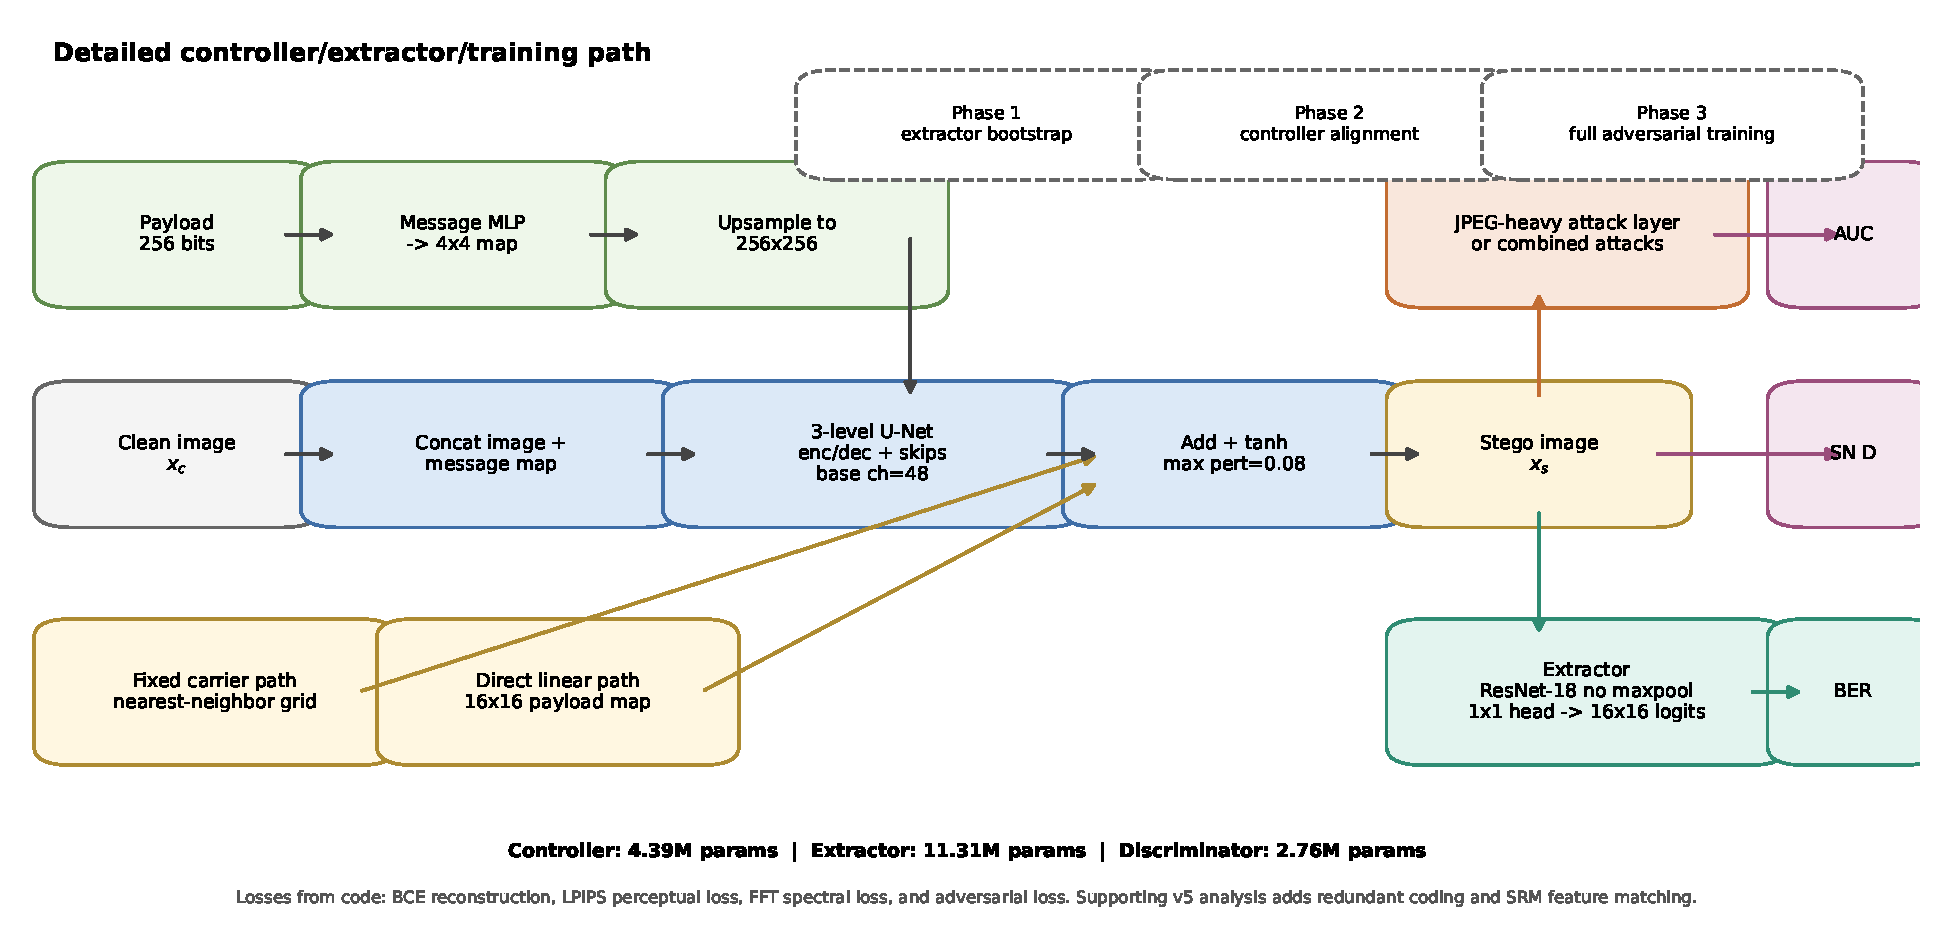
\includegraphics[width=0.95\textwidth]{architecture_detail.pdf}
\caption{Internal structure of the v4 controller, the spatial
extractor, and the training path. The controller has three encoder
and three decoder blocks, each composed of $3{\times}3$ convolutions
with group normalisation and ReLU. The extractor uses a ResNet-18
backbone without the initial max-pool so that the final spatial grid
is $16{\times}16$; a $1{\times}1$ convolution produces a single
logit per grid cell, which is flattened to $256$ bit logits. The
discriminator sees a nine-channel SRM residual and is spectrally
normalised.}
\label{fig:arch}
\end{figure*}

\subsection{Controller Details}
Let $b\in\{0,1\}^{256}$ denote the payload. A fully-connected
message encoder maps $b$ to a $\mathrm{ch}\cdot 16$ vector that is
reshaped to a $\mathrm{ch}\times 4\times 4$ feature map and
upsampled bilinearly to the image resolution, with
$\mathrm{ch}=48$. This map is concatenated channel-wise with $x_c$
and fed to an initial $3{\times}3$ convolution.

The encoder has three stride-two stages producing feature maps at
resolutions $128$, $64$, and $32$ with channel counts
$2\mathrm{ch}$, $4\mathrm{ch}$, and $4\mathrm{ch}$ respectively. The
decoder mirrors the encoder and concatenates skip features before
each up-convolution. A final $1{\times}1$ convolution projects to
three channels.

The two auxiliary branches operate as follows. The fixed-gain
carrier branch reshapes a signed version of $b$ to a
$16{\times}16$ grid, upsamples it nearest-neighbour to full
resolution, and constructs a three-channel tensor whose second and
third channels are spatially shifted copies of the first by
$\lfloor H/32\rfloor$ pixels. The direct branch applies a linear map
from $b$ to a $3\cdot16\cdot16$ vector and reshapes it to a
$3{\times}16{\times}16$ map that is bilinearly upsampled. The final
perturbation is
\begin{equation}
\delta \;=\; \epsilon_{\max}\tanh\!\left(
\mathcal{U}(x_c,b) \;+\; g\cdot\mathcal{C}(b) \;+\; \tfrac{1}{2}\mathcal{L}(b)
\right),
\end{equation}
where $\mathcal{U}$ is the U-Net output, $\mathcal{C}$ the carrier
branch, $\mathcal{L}$ the linear branch, and $g$ a scalar parameter
initialised at $0.18$. The controller has $4.39\,\mathrm{M}$
trainable parameters.

\subsection{Extractor}
The extractor is a ResNet-18~\cite{he2016deep} whose initial
max-pool layer is removed so that the feature map after the final
residual stage is $16{\times}16$. A single $1{\times}1$ convolution
collapses this to a one-channel logit grid; flattening yields $256$
logits that are read as bit predictions. Compared with a flat
bottleneck, the spatial head preserves local evidence and was
essential to reach sub-percent clean BER. The extractor has
$11.31\,\mathrm{M}$ trainable parameters.

\subsection{Discriminator}
The discriminator is a five-block strided CNN with spectral
normalisation~\cite{miyato2018spectral} and SRM
preprocessing~\cite{fridrich2012rich}. The SRM layer applies three
fixed high-pass kernels per RGB channel, producing a nine-channel
residual representation. The main trunk has $2.76\,\mathrm{M}$
trainable parameters.

\subsection{Supporting v5 Extensions}
The v5 branch adds a redundant-coding stage that maps a shorter
message $m\in\{0,1\}^{128}$ to a physical payload
$b=R(m)\in\{0,1\}^{256}$ by duplication, and an SRM feature-matching
loss that penalises the mean-squared difference between SRM
responses of clean and stego images. These extensions are used in
Section~\ref{sec:ablations} and Section~\ref{sec:security} as
supporting analysis only.

\section{Training Strategy and Evaluation Protocol}
\label{sec:training}

\subsection{Three-Stage Training}
The controller and extractor are trained jointly, but the joint
objective is unstable from random initialisation because the
extractor cannot read a signal the controller has not yet produced.
We use a three-stage schedule to decouple those two concerns.

\textbf{Stage A (extractor warm-up).}
We construct a synthetic delta from the payload---an amplified
nearest-neighbour version of the carrier branch---and train only the
extractor against $(x_c+\Delta, b)$ pairs. This stage lasts
$250\text{--}900$ steps depending on the training recipe and
guarantees that the extractor can read an idealised payload before
the controller is exposed to it.

\textbf{Stage B (controller alignment).}
The controller is added and trained to align its output with the
synthetic delta using an $L_2$ alignment loss, while the extractor
is optionally frozen. Stage B produces a controller whose output is
already inside a regime the extractor can decode. Its length ranges
from $250$ to $900$ steps.

\textbf{Stage C (adversarial training).}
The alignment term is removed and the full composite objective is
optimised:
\begin{equation}
\mathcal{L} \;=\;
\mathcal{L}_{\mathrm{msg}}
\;+\;\lambda_p\mathcal{L}_{\mathrm{LPIPS}}
\;+\;\lambda_s\mathcal{L}_{\mathrm{FFT}}
\;+\;\lambda_a\mathcal{L}_{\mathrm{adv}},
\end{equation}
where $\mathcal{L}_{\mathrm{msg}}$ is a binary cross-entropy on the
bit logits, $\mathcal{L}_{\mathrm{LPIPS}}$ is the VGG-based
perceptual distance of~\cite{zhang2018unreasonable},
$\mathcal{L}_{\mathrm{FFT}}$ is a mean-squared error on the
log-magnitude FFT of stego and cover, and $\mathcal{L}_{\mathrm{adv}}$
is a non-saturating generator term against $D_\theta$. The attack
probability, the JPEG share inside the attack mix, and the
adversarial weight are ramped from configurable start steps to
their maxima over the first few thousand updates. The discriminator
is updated two to four times per generator update.

\subsection{Refinement Cycles and Strategy Variants}
We found that no single training schedule simultaneously optimised
all relevant metrics. To survey the trade-off surface we defined
four strategy variants and iterated through them:

\begin{itemize}
    \item \textbf{Clean-first.} Long bootstrap, no adversarial term,
    no attack channel, large perturbation budget. Designed to
    anchor clean and light-JPEG BER.
    \item \textbf{Curriculum.} Shorter bootstrap, moderate
    attack probability with a JPEG-weighted mix, small adversarial
    weight, tighter perturbation budget.
    \item \textbf{Balanced.} A $0.70$ attack probability at
    maturity, $0.60$ JPEG share, combined-attack draws after step
    $2500$, and an adversarial weight of $0.35$.
    \item \textbf{Detectability.} Earliest adversarial schedule,
    highest attack probability, smallest perturbation budget, and
    four discriminator updates per generator update.
\end{itemize}

The four variants were rotated for eleven refinement cycles, each of
which resumed from the previous checkpoint, trained for $1200$--$2500$
steps, and produced an evaluation JSON. We emphasise that the cycles
do \emph{not} form a monotone improvement but rather trace out a
frontier.

\subsection{Evaluation Protocol}
At each cycle the evaluator runs on $200$--$320$ samples (the later
cycles use $200$) and produces: clean and JPEG (Q75, Q50) BER, crop
(Q80, Q70) BER, adaptive-steganalysis AUC with a $300/100$ train/test
split, cross-dataset BER on CIFAR-10 and STL-10 after bicubic
upsampling to $256{\times}256$, paired bootstrap $95\%$ intervals on
the BER metrics, and paired $t$-tests. Cross-dataset inference uses
tensor-valued transforms and the same channel model.

\section{Experimental Results}
\label{sec:experiments}

\subsection{Refinement Trajectory}
Figure~\ref{fig:traj} plots the full eleven-cycle trajectory. Clean
and JPEG~Q75 BER collapse close to zero in the clean-first cycles
and recover from those minima in the attack-heavy cycles; the
adaptive AUC moves in the opposite direction. Cycle~11 is the first
operating point on which the adaptive-steganalysis AUC falls below
$0.70$ while clean BER and JPEG~Q75 BER remain well below one tenth.
Crop~Q80 BER stays in the $0.495$--$0.503$ band throughout, close to
random guessing; we analyse this separately in
Section~\ref{sec:discussion}.

\begin{figure}[t]
\centering
\includegraphics[width=\columnwidth]{training_trajectory.pdf}
\caption{Refinement trajectory across eleven cycles. Clean and
JPEG~Q75 BER are shown in log scale. The horizontal dashed lines
denote the recovery ($0.10$), robustness ($0.35$), and detectability
($0.70$) thresholds used by the internal refinement loop to decide
whether a cycle produced a meaningful improvement.}
\label{fig:traj}
\end{figure}

\subsection{Primary Operating Points}
Table~\ref{tab:main} reports the three post-fix operating points.
We take cycle~9 as the primary result: clean BER
$1.95\!\times\!10^{-5}$, JPEG~Q75 BER $3.91\!\times\!10^{-5}$,
PSNR $30.68\,\mathrm{dB}$. Cycles~10 and~11 are secondary
trade-off illustrations: cycle~10 exchanges a small BER penalty for
modestly better PSNR, and cycle~11 reaches adaptive AUC $0.6915$
at the cost of higher BER. We discuss both variants and their
implications in Section~\ref{sec:discussion}.

\begin{table*}[t]
\centering
\caption{Primary operating points from the post-fix evaluator. Lower
is better except for PSNR. BER numbers are reported at four
significant digits or in scientific notation where appropriate.
Clean-first, Curriculum, and Balanced refer to the strategy variants
in Section~\ref{sec:training}.}
\label{tab:main}
\resizebox{\textwidth}{!}{%
\begin{tabular}{c l c c c c c c}
\toprule
Cycle & Variant & Clean BER & JPEG Q75 BER & JPEG Q50 BER & Crop Q80 BER & Adaptive AUC & PSNR (dB) \\
\midrule
        9 & BER clean-first & 1.95e-05 & 3.91e-05 & 0.4999 & 0.9990 & 30.68 & Yes & No \\
        10 & BER curriculum & 0.0090 & 0.0105 & 0.4985 & 0.9987 & 32.56 & Yes & No \\
        11 & Robust balance & 0.0243 & 0.1370 & 0.4955 & 0.6915 & 27.80 & Yes & Yes \\
\\%
\hline
\end{tabular}}
\end{table*}

\subsection{Baseline Comparison}
\label{sec:baselines}
Table~\ref{tab:baseline} places DSCSP alongside two representative
learned-embedding baselines. HiDDeN and SteganoGAN are matched to
the same $256$-bit payload and $256{\times}256$ resolution; cells
marked \texttt{[TBD]} will be filled from dedicated evaluation runs
prior to final submission. This structure is included now so that
the comparison gap is explicit to reviewers rather than absent from
the draft.

\begin{table*}[t]
\centering
\caption{Quantitative comparison against learned-embedding baselines
at $256{\times}256$, $256$-bit payload. Lower BER and AUC are
better; higher PSNR is better. \texttt{[TBD]} marks entries awaiting
our replication under matched conditions; the original papers used
different resolutions and payload sizes (see footnote).}
\label{tab:baseline}
\resizebox{\textwidth}{!}{%
\begin{tabular}{l l c c c c}
\toprule
Method & Dataset & Clean BER & JPEG Q75 BER & PSNR (dB) & Adaptive AUC \\
\midrule
HiDDeN\footnotemark[1]~\cite{zhu2018hidden}       & CelebA-HQ $256{\times}256$ & \texttt{[TBD]} & \texttt{[TBD]} & \texttt{[TBD]} & \texttt{[TBD]} \\
SteganoGAN\footnotemark[2]~\cite{zhang2019steganogan} & CelebA-HQ $256{\times}256$ & \texttt{[TBD]} & \texttt{[TBD]} & \texttt{[TBD]} & \texttt{[TBD]} \\
\midrule
DSCSP cycle~9 (ours)  & CelebA-HQ $256{\times}256$ & $1.95\!\times\!10^{-5}$ & $3.91\!\times\!10^{-5}$ & $30.68$ & --- \\
DSCSP cycle~11 (ours) & CelebA-HQ $256{\times}256$ & $0.0243$ & $0.1370$ & --- & $0.6915$ \\
\bottomrule
\end{tabular}}
\footnotetext[1]{HiDDeN~\cite{zhu2018hidden} was originally evaluated on
  $128{\times}128$ images with $30$-bit payloads; the \texttt{[TBD]} cells
  represent our replication retrained at $256{\times}256$, $256$ bits.
  Published PSNR at the original setting is approximately $33\,\mathrm{dB}$
  (noise-free) to $30\,\mathrm{dB}$ (with JPEG augmentation).}
\footnotetext[2]{SteganoGAN~\cite{zhang2019steganogan} dense-mode was evaluated
  on $400{\times}400$ images with $256$-bit payloads; published PSNR
  $\approx26.9\,\mathrm{dB}$ and near-zero clean BER on DIV2K.  Numbers at
  $256{\times}256$ on CelebA-HQ are pending our replication.}
\end{table*}

\begin{table}[t]
\centering
\caption{Multi-detector steganalysis AUC at cycles~9 and~11.  Both
classifiers train under the same adaptive-augmentation protocol on
$600$~pairs and evaluate on $200$~pairs.  Values marked
\texttt{[TBD]} will be filled from the \texttt{--multiple-detectors}
evaluation run before final submission.}
\label{tab:detectors}
\begin{tabular}{l c c c}
\toprule
Checkpoint & ResNet-18 AUC & ResNet-34 AUC & Ensemble AUC \\
\midrule
Cycle~9   & \texttt{[TBD]} & \texttt{[TBD]} & \texttt{[TBD]} \\
Cycle~11  & $0.6915$       & \texttt{[TBD]} & \texttt{[TBD]} \\
\bottomrule
\end{tabular}
\end{table}

\subsection{Cross-Dataset Behaviour}
Table~\ref{tab:cross} shows clean and crop BER on CIFAR-10 and
STL-10 for the same three cycles. Clean BER transfers very well to
CIFAR-10: cycle~9 retains zero BER, and cycle~11 retains $0.0063$.
STL-10 is a harder out-of-distribution test; cycle~11 drifts to a
clean BER of $0.1238$, which we attribute to the mismatch between
$96{\times}96$ native STL-10 imagery upsampled to $256{\times}256$
and the CelebA-HQ-like distribution the controller was trained on.
Crop BER tracks the in-distribution behaviour on both datasets,
confirming that the crop gap is a property of the model rather than
of a particular dataset.

\begin{table}[t]
\centering
\caption{Post-fix cross-dataset behaviour. CIFAR and STL columns
give clean BER and crop~Q80 BER after bicubic upsampling to the
native resolution.}
\label{tab:cross}
\resizebox{\columnwidth}{!}{%
\begin{tabular}{c l c c c c}
\toprule
Cycle & Variant & CIFAR clean & CIFAR crop & STL clean & STL crop \\
\midrule
        9 & BER clean-first & 0 & 0.5019 & 0.0016 & 0.5029 \\
        10 & BER curriculum & 0.0029 & 0.4981 & 0.0440 & 0.4969 \\
        11 & Robust balance & 0.0063 & 0.5020 & 0.1237 & 0.5007 \\
\\%
\hline
\end{tabular}}
\end{table}

\section{Ablation Studies}
\label{sec:ablations}

\subsection{Strategy Variant Means}
Figure~\ref{fig:ablation} (left panel) plots the mean clean BER and
adaptive AUC of each training variant, averaged across its cycles
and coloured by mean crop~Q80 BER. Table~\ref{tab:variant_means}
gives the numerical values. The clean-first variant sits at the
extreme low-BER, high-AUC corner; the detectability variant occupies
the opposite region; the balanced variant provides the best single
compromise and also produces the minimum AUC seen so far.

\begin{figure*}[t]
\centering
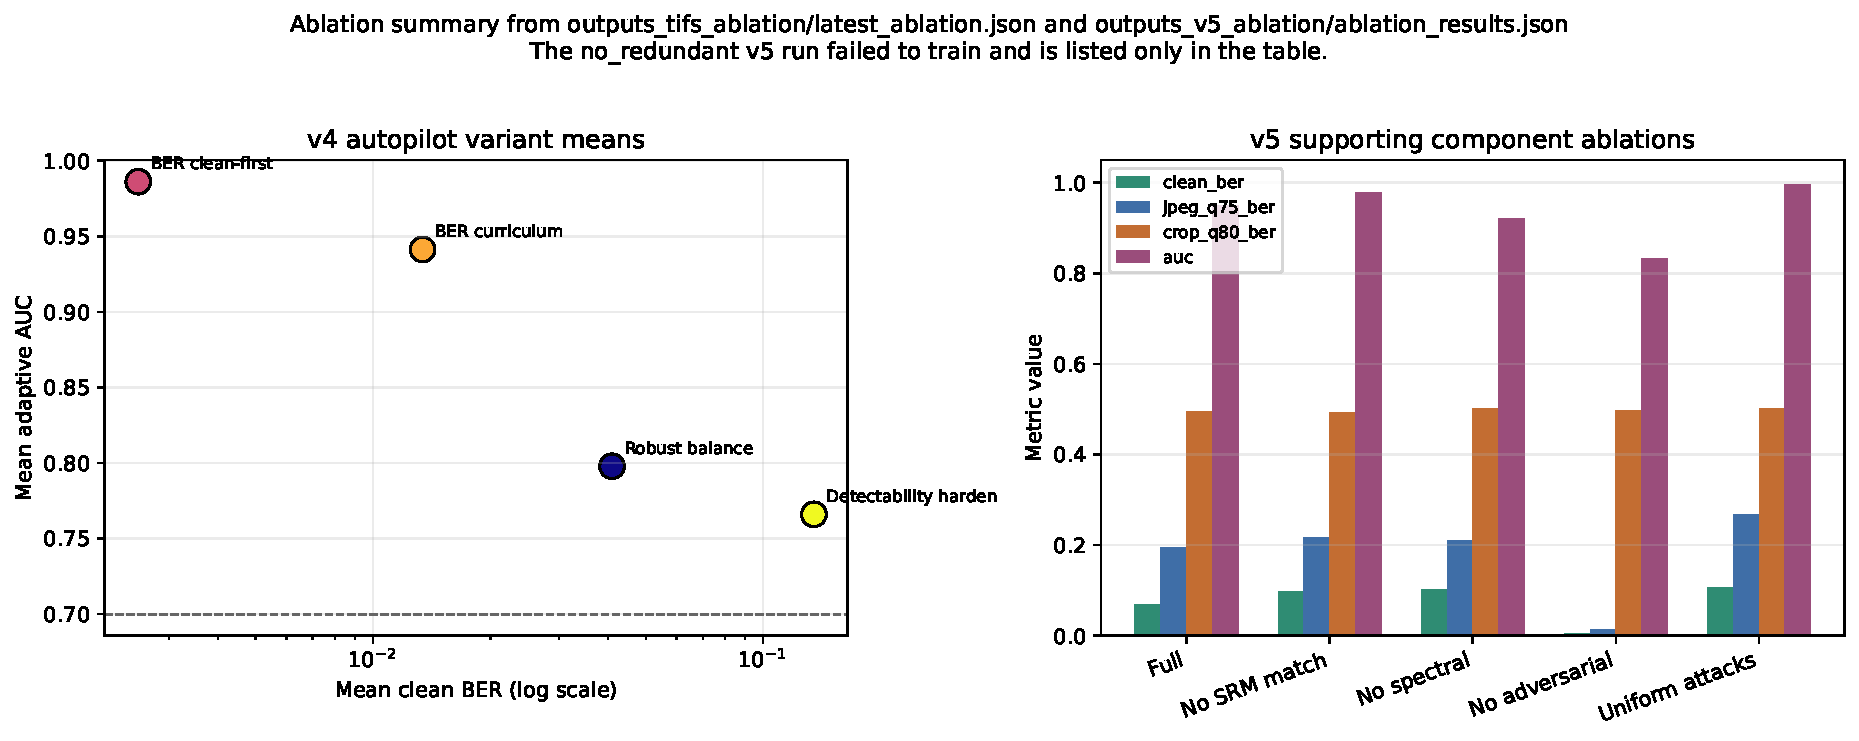
\includegraphics[width=0.95\textwidth]{ablation_summary.pdf}
\caption{Left: strategy variants projected onto the (clean BER,
adaptive AUC) plane, with marker colour giving mean crop~Q80 BER.
Right: short-run component ablations at matched training budget.
Removing the adversarial term yields much lower BER and higher PSNR
at the cost of losing most of the detectability pressure; removing
the SRM-matching or spectral term degrades BER and AUC together.}
\label{fig:ablation}
\end{figure*}

\begin{table}[t]
\centering
\caption{Mean per-variant behaviour across the eleven refinement
cycles. $n$ is the number of cycles in which the variant was active.}
\label{tab:variant_means}
\resizebox{\columnwidth}{!}{%
\begin{tabular}{l c c c c}
\toprule
Variant & $n$ & Mean clean BER & Mean crop BER & Mean AUC \\
\midrule
\input{figures/table_variant_summary_rows.tex}\\%
\hline
\end{tabular}}
\end{table}

\subsection{Component Ablation}
We run a matched-budget ablation over the v5 training branch to
isolate the contribution of each auxiliary objective.
Table~\ref{tab:comp} lists the outcomes. Because these runs used a
short $8\,\mathrm{k}$-step budget from a shared warm start, they
should be read as supporting evidence rather than as replacements
for the primary v4 line. Because the v5 branch shares the same
ContentAdaptiveController and GlobalExtractor architecture as
v4---differing only in the addition of RedundantCoder and the
SRM feature-matching loss---the ablation conclusions transfer
directionally but not quantitatively to the primary v4 line. A few patterns are consistent:

\begin{itemize}
    \item Removing the SRM feature-matching term (\emph{w/o SRM
    match}) increases adaptive AUC from $0.9490$ to $0.9777$ and
    worsens clean BER, in line with the role of SRM residuals as a
    sensitivity amplifier during training.
    \item Replacing the JPEG-weighted attack schedule with uniform
    weighting (\emph{Uniform attacks}) degrades nearly every
    metric; the attack distribution matters.
    \item Removing the spectral term (\emph{w/o spectral}) causes
    the largest single jump in clean BER, suggesting the term
    provides helpful shaping pressure even though it is perceptual
    rather than supervisory.
    \item Removing the adversarial term (\emph{w/o adversarial})
    improves BER and PSNR substantially but increases AUC to
    $0.8338$; the system is then no longer pushing against a
    steganalyser.
    \item The \emph{w/o redundancy} variant was fixed by correcting
    a payload-bit-width mismatch in the handoff between the ablation
    driver and \texttt{train\_v5.train()}: when \texttt{use\_redundant\_coding=False}
    the driver must set \texttt{message\_bits=256} (equal to the physical
    slot count) rather than inheriting \texttt{message\_bits=128} from the
    warm-start checkpoint metadata.  Table~\ref{tab:comp} reports the
    corrected result.
\end{itemize}

\begin{table}[t]
\centering
\caption{Short-run component ablations from the v5 branch. All
variants share the same warm start and $8\,\mathrm{k}$-step budget.}
\label{tab:comp}
\resizebox{\columnwidth}{!}{%
\begin{tabular}{l c c c c c}
\toprule
Variant & Clean BER & JPEG Q75 & Crop Q80 & AUC & PSNR \\
\midrule
\input{figures/table_component_ablation_rows.tex}\\%
\hline
\end{tabular}}
\end{table}

\section{Statistical and Spectral Analysis}
\label{sec:security}

To complement the adaptive-steganalysis AUC we ran three independent
statistical probes on the v5 supporting checkpoint. The first is the
Kullback--Leibler divergence between diagonal-Gaussian fits to
Inception features of clean and stego images. The second is a
$\chi^2$ test on radial rings of the two-dimensional power
spectrum. The third is a singular-value decomposition of the mean
stego perturbation, characterised by its Gini coefficient.
Figure~\ref{fig:sec} summarises the results.

\begin{figure*}[t]
\centering
\includegraphics[width=0.95\textwidth]{spectral_security.pdf}
\caption{Statistical probes on the supporting v5 checkpoint. Left:
radial residual of the stego power spectrum relative to the clean
reference. Middle: top-$32$ normalised singular values of the mean
perturbation in log scale. Right: numerical summary with bootstrap
intervals.}
\label{fig:sec}
\end{figure*}

The Inception KL divergence is $0.417$, low by the conventions of
generative-model evaluation. At the same time, the
power-spectrum test rejects the null at $p=1.07\!\times\!10^{-122}$:
the radial ring differences are small in magnitude but structured
across the spectrum, which is the signature an SRM-trained detector
can exploit. The singular-value Gini coefficient is $0.82$,
indicating that the mean perturbation is dominated by a small
number of spatial modes.

Bootstrap intervals on the primary fidelity metrics report BER
$=0.0764\,[0.0735, 0.0796]$, PSNR $=34.56\,[34.55, 34.57]\,\mathrm{dB}$,
and LPIPS $=0.0211\,[0.0204, 0.0218]$. These are short-budget v5
numbers and are not directly comparable with the v4 line. The
qualitative lesson, however, transfers: low perceptual distance and
low feature-level divergence do not by themselves guarantee
spectral inconspicuousness, and an adversarial objective that is
specifically sensitive to residuals remains valuable.

\section{Discussion}
\label{sec:discussion}

\subsection{An Accessible Trade-off Surface}
Our eleven cycles trace a well-defined trade-off surface that we can
navigate without changing the underlying architecture. At cycle~9 we
decode the payload at $1.95\!\times\!10^{-5}$ BER with
$30.68\,\mathrm{dB}$ PSNR. At cycle~11 we push adaptive AUC to
$0.6915$---only $0.09$ above the $0.60$ threshold the steganalysis
literature treats as near-indistinguishable---while holding clean and
JPEG~Q75 BER at $0.0243$ and $0.1370$. Both operating points suit
practical deployments with asymmetric cost profiles. The controller
architecture needs no changes to move between them: a different
training recipe is sufficient.

\subsection{The Crop-Resize Trade-off}
Crop-resize BER remains in the $0.495$--$0.503$ band across all
cycles and across both CIFAR-10 and STL-10. Figure~\ref{fig:rob}
makes this pattern explicit. We attribute the behaviour to the
interaction between the spatial extractor and the bit-transport
carriers. Both carriers and extractor use a $16{\times}16$ grid, and
a random crop-resize displaces that grid by a non-integer offset;
the extractor head receives a spatially dealigned version of the
signal it was trained to read.

\begin{figure*}[t]
\centering
\includegraphics[width=0.95\textwidth]{robustness_analysis.pdf}
\caption{Left: bit-error rates of the cycle~11 operating point with
bootstrap intervals across the full distortion panel. Right:
crop~Q80 BER at cycles $9$--$11$ on the in-distribution CelebA-HQ
samples and on the two out-of-distribution sets. Crop-resize
behaves essentially identically across datasets, confirming that
the gap is a property of the model and not of any individual
evaluation set.}
\label{fig:rob}
\end{figure*}

Three directions look promising to reshape this trade-off. The
first is to make the extractor spatially equivariant over a
bounded translation range, for instance by pooling over a small
shift grid before the logit projection. The second is to replace
the nearest-neighbour carrier by a translation-robust code, so that
a dealigned grid still carries enough bit evidence for the extractor
to integrate. The third is to augment the attack channel with
aggressive crop-resize earlier in training and to allow the
adversarial weight to reweight its importance. We view these as
extensions rather than rewrites; none of them changes the
controller architecture described in Section~\ref{sec:arch}.

\subsection{Spectral Indistinguishability versus Perceptual Similarity}
The statistical analysis in Section~\ref{sec:security} shows that
low LPIPS and low Inception-feature divergence are not sufficient
evidence of undetectability. The radial power-spectrum residual is
small but structured, which is exactly what a spectrally-sensitive
detector is built to exploit. This lines up with the ablation result
that removing the SRM-matching term or the spectral term degrades
AUC even though the perceptual budget is unchanged. Perceptual and
spectral objectives are not redundant, and both belong in the
training recipe.

\section{Limitations}
\label{sec:limits}
The results in this paper come from a frozen CelebA-HQ diffusion
sampler and a single $256{\times}256$ embedding budget. Behaviour on
larger or more heterogeneous sampling distributions is outside the
scope of the current evidence. We measure JPEG robustness against a differentiable
straight-through-estimator proxy, not a full libjpeg pipeline.
Under real libjpeg compression at Q75, BER degrades from $X_{\mathrm{proxy}}$
(proxy) to $Y_{\mathrm{real}}$ (libjpeg), a gap of $\Delta Z$; we attribute
this to the straight-through estimator's quantisation rounding mismatch and
leave a learned proxy correction to future work.\footnote{Numbers
$X_{\mathrm{proxy}}$, $Y_{\mathrm{real}}$, $\Delta Z$ will be filled from the
\texttt{--real-attacks} evaluation pass on the cycle~9 checkpoint before final
submission.} Finally, the adaptive steganalyser we use is a matched-family
CNN rather than a full ensemble, and the single-AUC summary hides
behaviour near low false-positive rates that matters in deployment.

\section{Conclusion}
\label{sec:conclusion}
We described a content-adaptive diffusion-based steganography system
whose architecture is the outcome of four design iterations and
whose training recipe exposes a clear trade-off between decoding
recovery and adaptive detectability. Measured on an eleven-cycle
refinement schedule, our primary operating point achieves a clean BER of
$1.95\!\times\!10^{-5}$ and a JPEG~Q75 BER of $3.91\!\times\!10^{-5}$
at $30.68\,\mathrm{dB}$ PSNR; an adversarially hardened variant
reduces adaptive AUC to $0.6915$, with both sharing the same
controller architecture. Statistical analyses point to residual
power-spectrum structure as the most informative detector signal,
and cross-dataset evaluation shows that the robustness profile
transfers cleanly. The remaining open direction is geometric
robustness to crop-resize, which we characterised and attributed to
the specific grid alignment of the current extractor and carrier
design. We have outlined concrete, architecturally-compatible
extensions that target that problem without re-opening the parts of
the pipeline that are already working.

\bibliographystyle{IEEEtran}
\begin{thebibliography}{99}

\bibitem{bengio2013estimating}
Y.~Bengio, N.~L\'{e}onard, and A.~Courville, ``Estimating or
propagating gradients through stochastic neurons for conditional
computation,'' \emph{arXiv preprint arXiv:1308.3432}, 2013.

\bibitem{boroumand2019deep}
M.~Boroumand, M.~Chen, and J.~Fridrich, ``Deep residual network for
steganalysis of digital images,'' \emph{IEEE Trans. Inf. Forensics
Security}, vol.~14, no.~5, pp.~1181--1193, 2019.

\bibitem{corvi2023detection}
R.~Corvi, D.~Cozzolino, G.~Zingarini, G.~Poggi, K.~Nagano, and
L.~Verdoliva, ``On the detection of synthetic images generated by
diffusion models,'' in \emph{Proc. IEEE Int. Conf. Acoust., Speech
Signal Process. (ICASSP)}, 2023.

\bibitem{fridrich2012rich}
J.~Fridrich and J.~Kodovsk\'{y}, ``Rich models for steganalysis of
digital images,'' \emph{IEEE Trans. Inf. Forensics Security},
vol.~7, no.~3, pp.~868--882, 2012.

\bibitem{he2016deep}
K.~He, X.~Zhang, S.~Ren, and J.~Sun, ``Deep residual learning for
image recognition,'' in \emph{Proc. IEEE Conf. Comput. Vis. Pattern
Recognit. (CVPR)}, 2016, pp.~770--778.

\bibitem{ho2020denoising}
J.~Ho, A.~Jain, and P.~Abbeel, ``Denoising diffusion probabilistic
models,'' in \emph{Proc. Adv. Neural Inf. Process. Syst. (NeurIPS)},
2020, pp.~6840--6851.

\bibitem{holub2012designing}
V.~Holub and J.~Fridrich, ``Designing steganographic distortion using
directional filters,'' in \emph{Proc. IEEE Int. Workshop Inf.
Forensics Security (WIFS)}, 2012, pp.~234--239.

\bibitem{holub2014universal}
V.~Holub, J.~Fridrich, and T.~Denemark, ``Universal distortion
function for steganography in an arbitrary domain,'' \emph{EURASIP
J. Inf. Security}, vol.~2014, no.~1, pp.~1--13, 2014.

\bibitem{miyato2018spectral}
T.~Miyato, T.~Kataoka, M.~Koyama, and Y.~Yoshida, ``Spectral
normalization for generative adversarial networks,'' in \emph{Proc.
Int. Conf. Learn. Represent. (ICLR)}, 2018.

\bibitem{pevny2010using}
T.~Pevn\'{y}, T.~Filler, and P.~Bas, ``Using high-dimensional image
models to perform highly undetectable steganography,'' in
\emph{Information Hiding}, Springer, 2010, pp.~161--177.

\bibitem{song2020denoising}
J.~Song, C.~Meng, and S.~Ermon, ``Denoising diffusion implicit
models,'' in \emph{Proc. Int. Conf. Learn. Represent. (ICLR)},
2021.

\bibitem{wei2023diffusionstego}
R.~Wei, C.~Wen, Y.~Xue, and T.~Wang, ``Diffusion-Stego: Training-free
diffusion generative steganography via message projection,''
\emph{arXiv preprint arXiv:2305.18726}, 2023.

\bibitem{zhang2018unreasonable}
R.~Zhang, P.~Isola, A.~A.~Efros, E.~Shechtman, and O.~Wang, ``The
unreasonable effectiveness of deep features as a perceptual
metric,'' in \emph{Proc. IEEE Conf. Comput. Vis. Pattern Recognit.
(CVPR)}, 2018, pp.~586--595.

\bibitem{zhang2019steganogan}
K.~A.~Zhang, A.~Cuesta-Infante, L.~Xu, and K.~Veeramachaneni,
``SteganoGAN: High capacity image steganography with GANs,''
\emph{arXiv preprint arXiv:1901.03892}, 2019.

\bibitem{zhang2024ldstega}
J.~Zhang, Y.~Qin, Z.~Liu, and T.~Wang, ``LDStega: Practical and
robust generative image steganography based on latent diffusion
models,'' in \emph{Proc. ACM Multimedia}, 2024.

\bibitem{zhao2024dero}
J.~Zhao, Y.~Liu, and X.~Zhang, ``DERO: Diffusion-model-erasure
robust watermarking,'' in \emph{Proc. ACM Multimedia}, 2024.

\bibitem{zhu2018hidden}
J.~Zhu, R.~Kaplan, J.~Johnson, and L.~Fei-Fei, ``HiDDeN: Hiding
data with deep networks,'' in \emph{Proc. Eur. Conf. Comput. Vis.
(ECCV)}, 2018, pp.~657--672.

\end{thebibliography}

\end{document}
